\documentclass[border=0.1cm]{standalone}
\usepackage[utf8]{inputenc}

\usepackage{tikz}
\usepackage{amsfonts}
\usepackage{amsmath,amssymb}
\usepackage{systeme,mathtools}
\usetikzlibrary{positioning,arrows.meta,quotes}
\usetikzlibrary{shapes,snakes}
\usetikzlibrary{bayesnet}
\tikzset{>=latex}

\begin{document}
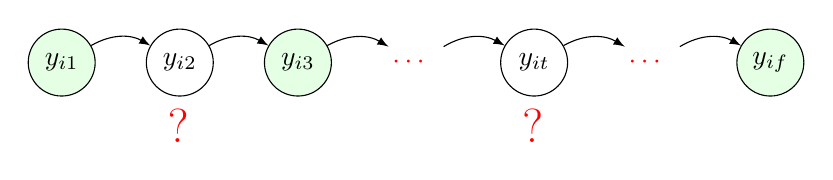
\begin{tikzpicture}
\node[circle,draw=black,fill=green!10,inner sep=0pt,minimum size=0.85cm] (obs1) at (0,0) {$y_{i1}$};
\node[circle,draw=black,fill=white,inner sep=0pt,minimum size=0.85cm] (obs2) at (1.5,0) {$y_{i2}$};
\node[circle,draw=black,fill=green!10,inner sep=0pt,minimum size=0.85cm] (obs3) at (3,0) {$y_{i3}$};
\node[text width=0.6cm] (obs4) at (4.5,0) {\color{red}{$\LARGE\cdots$}};
\node[circle,draw=black,fill=white,inner sep=0pt,minimum size=0.85cm] (obs5) at (6,0) {$y_{it}$};
\node[text width=0.6cm] (obs6) at (7.5,0) {\color{red}{$\LARGE\cdots$}};
\node[circle,draw=black,fill=green!10,inner sep=0pt,minimum size=0.85cm] (obs7) at (9,0) {$y_{if}$};
\path [draw,->] (obs1) edge [bend left] node [right] {} (obs2);
\path [draw,->] (obs2) edge [bend left] node [right] {} (obs3);
\path [draw,->] (obs3) edge [bend left] node [right] {} (obs4);
\path [draw,->] (obs4) edge [bend left] node [right] {} (obs5);
\path [draw,->] (obs5) edge [bend left] node [right] {} (obs6);
\path [draw,->] (obs6) edge [bend left] node [right] {} (obs7);
\node[text width=0.3cm] (unknown1) at (1.5,-0.8) {\LARGE\color{red}{?}};
\node[text width=0.3cm] (unknown1) at (6,-0.8) {\LARGE\color{red}{?}};
\end{tikzpicture}
\end{document}
